%%=============================================================================
%% POC
%%=============================================================================
\chapter{\IfLanguageName{dutch}{Proof Of Concept}{Proof Of Concept}}%
\label{ch:poc}

Als technische component binnen deze studie wordt er een proof of concept uitgewerkt waarbij we de firmware van een HA firewall pair die zich bevindt binnen een actieve productiesite van VPK Packaging Group gaan updaten zonder dat er zich enige vorm van downtime voordoet in de productie. Met als doel hiervan het 

Er werd gekozen om te werken met de Palo Alto PA-440 firewalls, enerzijds omdat deze binnen VPK worden gebruikt binnen de verschillende productiesites en zo dus een waarheidsgetrouw en nuttig beeld geven van de zaken die moeten worden uitgevoerd om een HA firewall pair te upgraden.

Als technische component binnen deze studie wordt een proof of concept uitgewerkt waarin de firmware -upgrade van een HA firewall pair in een actieve productiesite van VPK Packaging Group wordt gedemonstreerd. Het doel hiervan is op een representatieve en gecontroleerde manier aan te tonen hoe een dergelijke upgrade kan worden uitgevoerd zonder enige vorm van downtime in de productieomgeving. Hierbij wordt niet enkel aandacht besteed aan het technische proces van de upgrade zelf, maar ook aan de reproduceerbaarheid ervan binnen andere nieuwe productiesites die VPK later mogelijks zal aankopen.


\section{Financiële impact van downtime binnen twee VPK sites}
Er kan niet genoeg benadrukt worden dat deze POC van uitzonderlijke waarde is voor VPK. De kleinste afwijking of vergissing tijdens het upgraden van het HA-firewallpair kan immers catastrofale gevolgen hebben voor de organisatie. Om deze impact concreet te maken, kunnen we een inschatting maken van het financiële verlies per uur voor twee VPK-sites: Alizay en Oudegem.



\vspace{5mm}
\begin{table}[h!]
    \centering
    \resizebox{0.6\textwidth}{!}{%
        \begin{tabular}{|l|l|l|}
            \hline
            \textbf{Parameter} & \textbf{VPK Alizay} & \textbf{VPK Oudegem} \\
            \hline
            Gemiddeld jaaromzet (€) & 250.000.000 & 350.000.000 \\
            Aantal gewerkte uren per jaar& 5.650 uur & 5.650 uur \\
            \hline
        \end{tabular}%
    }
    \caption{Overzicht van financiële parameters voor VPK Alizay en VPK Oudegem.}
    \label{fig:VPKsites}
\end{table}


Het verwachte omzetverlies per uur tijdens downtime kunnen we eenvoudig berekenen met de volgende formule, waarbij de jaaromzet wordt gedeeld door het aantal uren dat de site produceert:

\[
\text{Omzetverlies per uur} = \frac{\text{Jaaromzet}}{\text{Gewerkte uren per jaar}}
\]
\vspace{5mm}

Voor de twee sites resulteert dit in de volgende berekeningen:

\vspace{5mm}
\[
\text{Omzetverlies per uur Alizay} = \frac{250.000.000}{5.650} = €44.247
\]

\[
\text{Omzetverlies per uur Oudegem} = \frac{350.000.000}{5.650} = €61.946
\]

Deze cijfers illustreren duidelijk hoe cruciaal het is om de upgrade zorgvuldig en zonder fouten uit te voeren, gezien de aanzienlijke financiële impact van zelfs een korte downtime.


\section{Beste High Availability settings voor de Palo Alto firewalls van FR16.}


High Availability (HA) is een functie die verschillende netwerk apparatuur vendors aanbieden, deze functie zorgt ervoor dat de downtime geminimaliseerd wordt door het gebruiken van meerdere entiteiten van dezelfde appartuur. Vaak zal er gebruik worden gemaakt van twee apparaten die dan op verschillende mogelijke manieren geconfigureerd kunnen worden. 

\vspace{5mm}Twee populaire manieren om deze apparaten te configurenen zijn Active/Active of Active/Passive. De termen Active en Passive slaan hier op de staat van het apparaat. Active betekend dat dit apparaat wel degelijk bepaalde netwerk functies op zich zal nemen en dus actief zal meerwerken om bepaalde data te verwerken. Passive betekend dat het apparaat niet actief data zal verwerken, en zich dus in een soort van rust stand bevindt.

\subsection{Active/Active firewall opstelling}
Bij een Active/Active opstelling verwerken beide apparaten actief data. In dit geval zullen beide firewalls gelijktijdig verkeer filteren op basis van vooraf gedefinieerde firewallregels. Hoewel dit in sommige situaties voordelen kan bieden, is deze opstelling in onze omgeving minder geschikt om meerdere redenen.
\newline



\begin{itemize}
    \item \textbf{Active/Active firewall pairs zijn complex om te installeren en onderhouden:}  Sessie synchronisatie tussen de firewalls kan complex worden, zeker als er gebruik wordt gemaakt van dynamische IP’s binnen het netwerk. Omdat er is besloten in bovenstaande rasci matrix dat het beheer van de OT firewall een verantwoorddelijkheid is van het OT team lijkt het niet verstandig om gebruik te maken van een complexe firewall opstelling omdat de kennis over het beheer van dit soort opstellingen minder groot is bij het OT team. 
    
    \item \textbf{Kans op asymmetrische sessies:} De kans is groter dat beide firewalls onafhankelijk data forwarden, waardoor inbound verkeer via een ander pad kan terugkeren dan outbound verkeer. Dit kan leiden tot session mismatches, met als gevolg dat data mogelijk wordt gedropt.
    
    \item \textbf{Inconsistentie met andere sites:}  Alle andere VPK-sites met een Palo Alto firewall-pair gebruiken een Active/Passive-opstelling. Een Active/Active-configuratie binnen FR16 zou de uniformiteit van de netwerkarchitectuur verstoren.
    
\end{itemize}

Ook is binnen deze Active/Active opstelling de mogelijkheid om gebruik te maken van parallel processing. Dit zorgt er effectief voor dat throughput verdubbeld wordt. \autocite{Fulp2006} Voor onze use case is dit echter niet relevant. De hoeveelheid data die via de Sophos firewall wordt verstuurd, is zo laag dat één Palo Alto firewall ruim voldoende capaciteit heeft om deze load zonder merkbare vertraging te verwerken. Uit een uitgebreide analyse van het netwerkverkeer op de WAN poort van de Sophos firewall, uitgevoerd over meerdere weken en op verschillende tijdstippen, blijkt dat de maximale gemeten throughput slechts 10 KBps bedroeg.

\vspace{5mm}
De nieuwe Palo Alto firewall (PA-440) zou een maximale throughput van 2,6 Gbps hebben en ondersteunt 200.000 gelijktijdige sessies. \autocite{PaloAltoDS2025} Dit betekent dat de beschikbare capaciteit ruimschoots volstaat en dat een Active/Active configuratie geen toegevoegde waarde biedt voor deze specifieke productiesite.

\begin{figure}[H]
    \centering
    \fbox{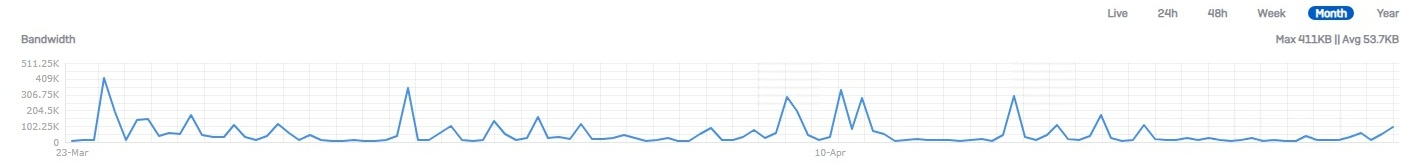
\includegraphics[scale=0.41]{fotos/SophosBandWidth.jpg}}
    \caption[Sophos firewall bandwidth graph]{\label{fig:grail}Totale bandbreedte die gebruikt wordt door de Sophos OT firewall van de productiesite van FR16}
\end{figure}




\subsection{Active/Passive firewall opstelling}

In een Active/Passive-opstelling is er slechts één firewall die gelijktijdig data verwerkt. Dit wordt mogelijk gemaakt door het configureren van HA-links. Deze links zijn cruciaal voor het waarborgen van redundantie, hoge prestaties en synchronisatie tussen firewalls in een HA-pair. Ze stellen de firewalls in staat om met elkaar te communiceren en statusinformatie te delen. Hierdoor kan de passieve firewall moeiteloos de taak van de actieve firewall overnemen bij een eventuele uitval. Zo zorgt de actieve firewall ervoor dat sessie-informatie wordt gedeeld met de passieve firewall, zodat deze altijd over de benodigde sessiegegevens beschikt in het geval van een failover. \autocite{PaloAltoHA2025} \autocite{PaloAltoHAb2025}

Verder in dit hoofdstuk zal een HA verbinding tussen twee firewalls worden geconfigureerd op basis van de behoeften van VPK en de algemene best practices.

\begin{figure}[H]
    \centering
    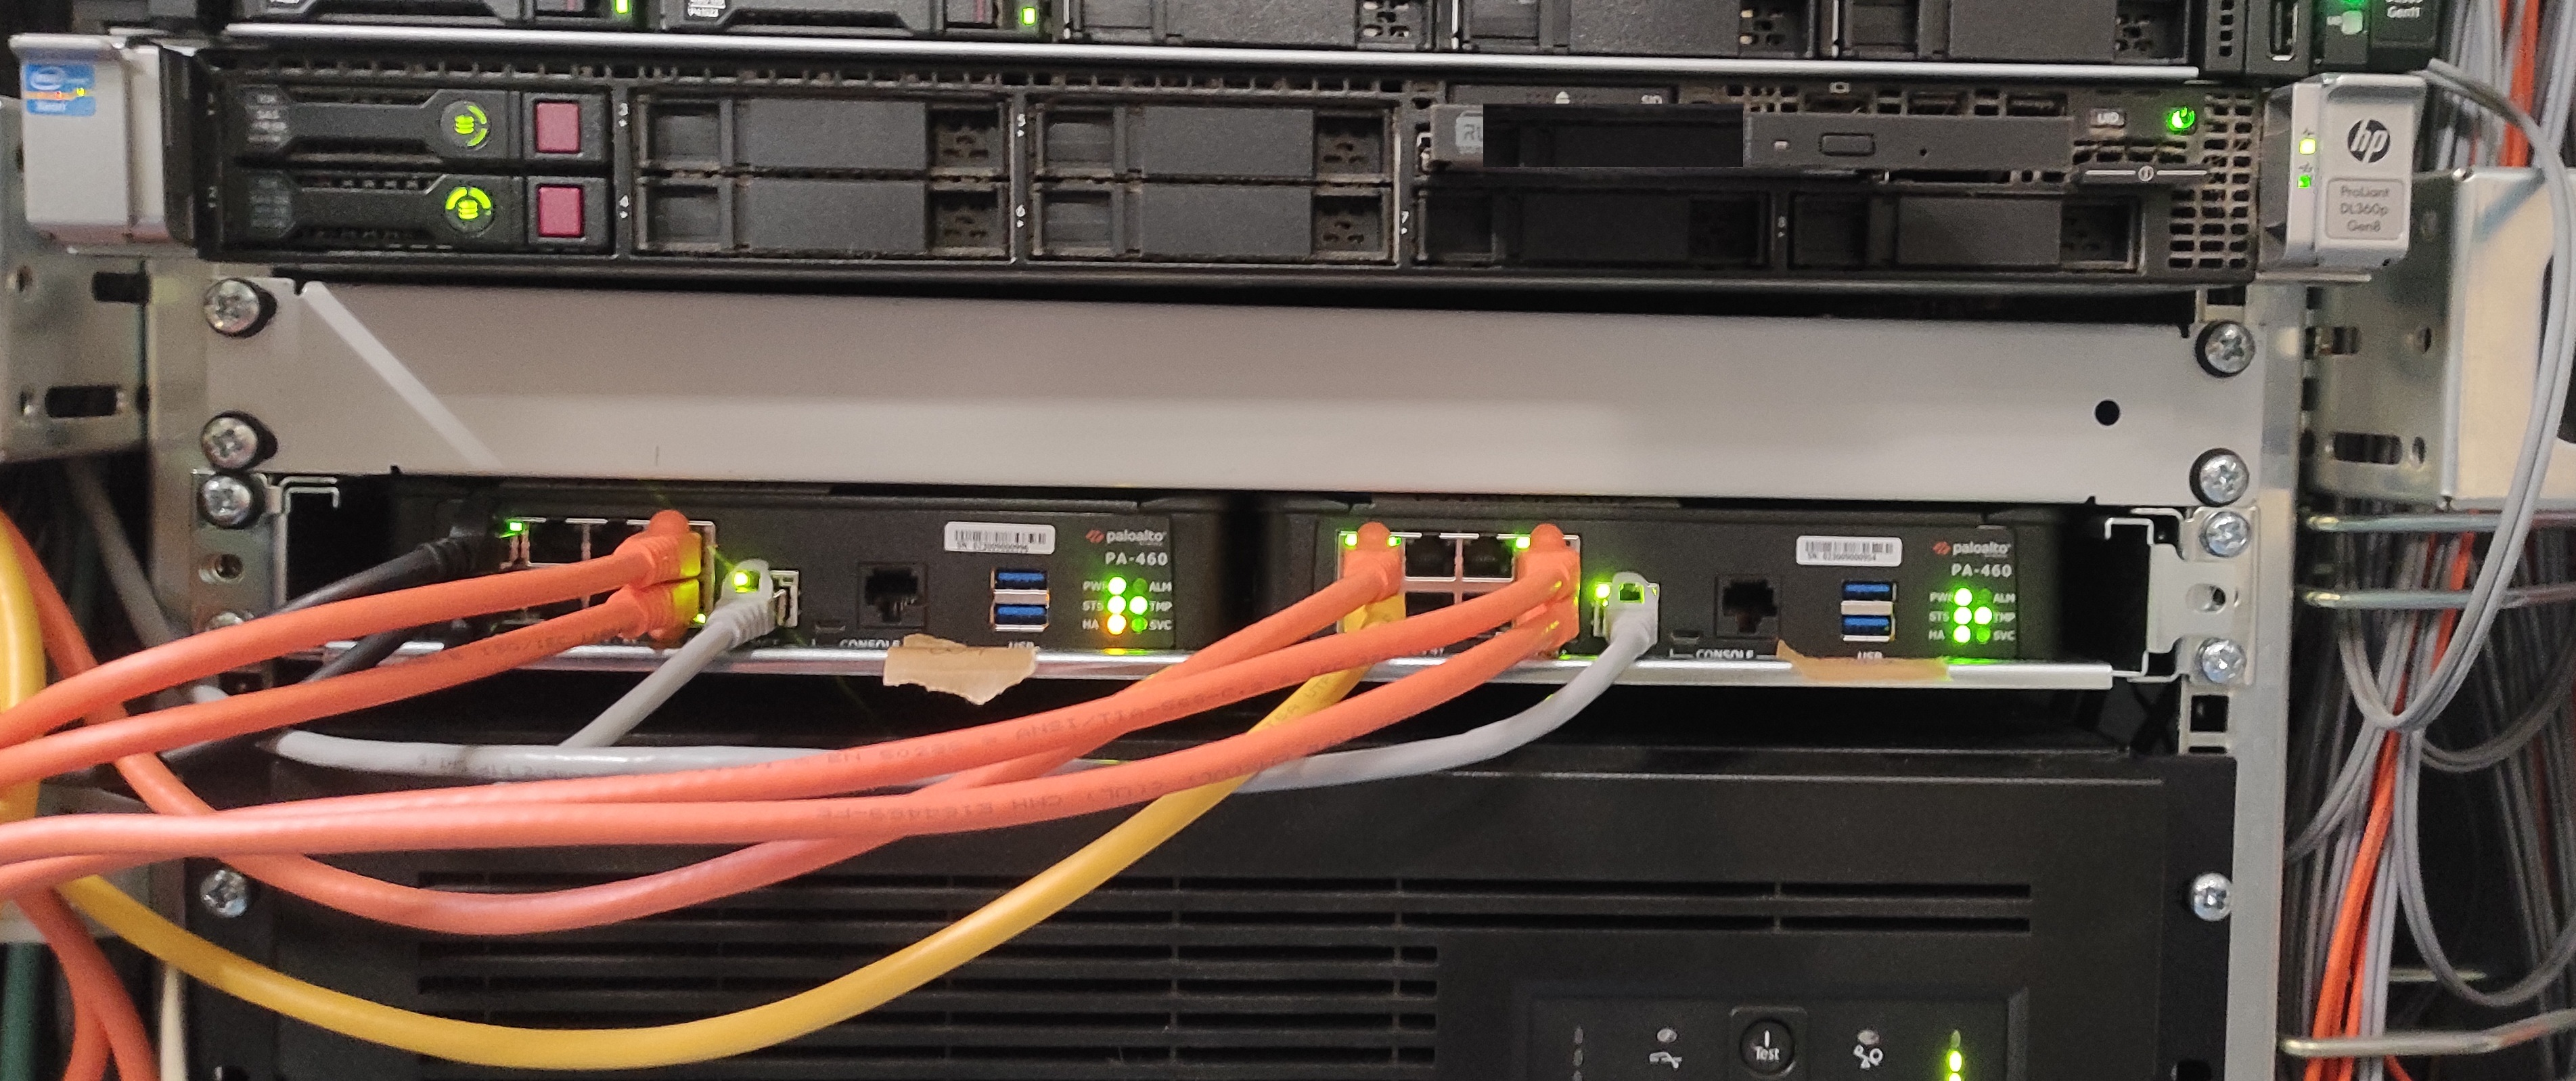
\includegraphics[width=0.8\textwidth]{fotos/PA_FirewallPairBE02.jpg}
    \caption[Palo Alto Active/Passive pair]{\label{fig:grail}Een Palo Alto Active/Passive firewall opstelling in de VPK site van Erembodegem.}
\end{figure} 



\section{Beste High Availability settings voor de Sophos firewall van FR16}

Om gebruik te kunnen maken van de HA-functies van de Sophos firewall is het noodzakelijk om twee identieke firewalls aan te schaffen. Momenteel is er echter slechts één firewall aanwezig, waardoor VPK genoodzaakt zal zijn om een tweede Sophos firewall aan te kopen om HA te kunnen implementeren. Dit proces is echter niet eenvoudig, aangezien het onduidelijk is hoe de huidige Sophos firewall is geconfigureerd. Als de twee firewalls in het HA-paar verschillende instellingen hebben, kan dit in de toekomst mogelijk problemen veroorzaken. Daarom moet er een tweede identieke firewall worden aangeschaft, en is het essentieel om een onderzoek te doen naar de huidige configuratie van de Sophos firewall.

\section{Configuratie van HA op een Palo Alto Firewall}

\textbf{Mode}
\begin{itemize}[label=\textbullet]
    \item Zoals eerder in dit hoofdstuk besproken is zal er bij de configuratie van een Palo Alto firewall pair binnen een VPK site gebruik worden gemaakt van een Active/Passive opstelling. Hierbij zal er steeds slechts één firewall tegelijk actief zijn.
\end{itemize}



\textbf{Enable Config Sync}
\begin{itemize}[label=\textbullet]
    \item Configuration synchronization is een setting binnen Palo Alto HA firewall pairs. Waarbij een groot aantal settings automatisch worden gesyncroniseerd tussen devices. Om conflicten in configuraties te vermijden is het steeds aangeraden om configuraties steeds op de Active firewall uit te voeren en te wachten tot de Passive firewall gesynced is. Een aantal settings die niet worden gesynchroniseerd zijn: content updates, HA settings, mgmt interface settings, \ldots 
\end{itemize}



\textbf{Passive Link state}
\begin{itemize}[label=\textbullet]
    \item Deze settings zal bepalen in welke status alle data interfaces van een Passive firewall zullen worden geplaatst. Bij het gebruiken van de `shutdown` modus zullen alle data interfaces op de passive firewall in een `down` state worden geplaatst. Naast deze modus is er ook de `auto` modus. Bij deze modus zal alle data interfaces op `up` laten staan, maar dropped alle packets die over deze interfaces zouden passeren. 
    
    \vspace{5mm}
    Echter zou dit er voor kunnen zorgen dat switches nog steeds data packets zouden versturen over deze schijnbare `up` interfaces. Dit probleem samen met de algemene beste hardening cybersecurity practices om alle poorten die niet gebruikt worden op `down` te zetten zorgt ervoor dat VPK gebruik zal maken van de `shutdown` modus op beide firewalls.
\end{itemize}



\textbf{Monitor fail hold down time}
\begin{itemize}[label=\textbullet]
    \item De ``monitor fail hold down time'' is een vooraf ingestelde timer om onnodige failover te voorkomen. Nadat één van de links down gaat zal het process geen nieuwe failover toestaan als het ziet dat er binnen de tijdslimiet van één minuut de interface terug `up` is. Mocht de link toch langer dan één minuut down zijn zal er toch een failover gebeuren. Binnen iedere andere firewall op een VPK site wordt deze zelfde timer gebruikt. Daarom is er in het belang van uniformiteit gekozen om ook op deze site de timer in te stellen op één minuut.
\end{itemize}



\textbf{Device Priority}
\begin{itemize}[label=\textbullet]
    \item Deze settings zal bepalen welke prioriteit een bepaalde firewall heeft binnen een HA firewall pair. Een hogere waarde betekent direct ook een hogere prioriteit. Echter is dit enkel nuttig als men gebruik maakt van preemption. Maar aangezien preemption uit staat op deze firewalls zal deze priority waarde dus geen nut hebben.
\end{itemize}



\textbf{Preemptive}
\begin{itemize}[label=\textbullet]
    \item Deze setting zal er voor zorgen dat de firewall met een hogere prioriteit in staat is om terug Active te worden nadat er een failover is gebeurd. Echter heeft VPK gekozen om deze setting niet in te schakelen bij alle firewalls op alle VPK sites.
\end{itemize}



\textbf{Hearbeat backup}
\begin{itemize}[label=\textbullet]
    \item Deze optie zorgt ervoor dat er een backup is om de hearbeat berichten van de apparaten op te sturen via de management interfaces van de firewall. Deze berichten zullen standaard over de HA1 en HA2 link worden verstuurd. Aangezien er twee rechtstreekse linken zijn tussen de twee firewalls in het HA pair is het dus niet meer nodig om deze optie aan te zetten.
\end{itemize}


\begin{figure}[H]
    \centering
    \fbox{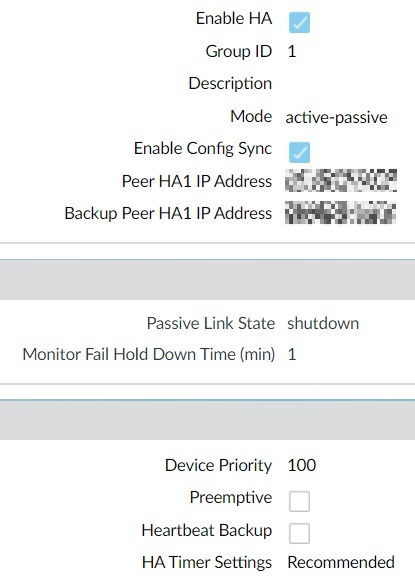
\includegraphics[scale=0.666]{fotos/PA_HASettings.jpg}}
    \caption[PA High Availability settings]{\label{fig:PA_HASettings}GUI (Graphical User Interface) interface om de settings om de configuratie van High Availability op een PA firewall aan te passen.}
\end{figure}

\section{Bepalen van het Palo Alto `upgrade path`}

Palo Alto NGFW's draaien op een besturingssysteem genaamd PAN-OS. Dit besturingssysteem wordt regelmatig bijgewerkt met nieuwe versies die verbeterde functionaliteiten, beveiligingsupdates en prestatieverbeteringen bevatten.

Bij het upgraden van een Palo Alto NGFW is niet altijd mogelijk om rechtstreeks van een oudere versie van PAN-OS naar de nieuwste versie over te stappen. Dit komt doordat grotere versies vaak significante wijzigingen bevatten in de onderliggende architectuur. Om de stabiliteit van het systeem te waarborgen, vereist Palo Alto Networks dat upgrades in specifieke stappen worden uitgevoerd. Dit pad van opeenvolgende versies wordt aangeduid als het upgrade path.

In figuur 
\begin{figure}[H]
    \centering
    \fbox{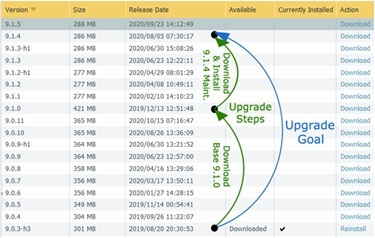
\includegraphics[scale=0.666]{fotos/UpgradePath.jpg}}
    \caption[PA High Availability settings]{\label{fig:UpgradePath} Een voorbeeld van een upgrade path dat gebruikt wordt om van PAN-OS versie 9.0.3-h3 naar versie 9.1.5 te upgraden. Bron: \cite{firewallcx2025}}
\end{figure}

\section{Verschilende soorten updates}
\subsection{Verschilende soorten software updates}
Palo Alto brengt wekelijks nieuwe OS updates uit voor PAN-OS. Deze updates zijn onderverdeeld in verschillende categorieën, elk met een specifiek doel en een eigen stabiliteitsniveau. Een goed begrip van deze release typen is essentieel om upgrades zorgvuldig te plannen en de continuïteit en beveiliging van het netwerk te waarborgen.

\vspace{5mm}
Een major release, zoals de overgang van PAN-OS 11.1 naar 11.2, introduceert vaak nieuwe functies, prestatieverbeteringen en ingrijpende wijzigingen in de systeemarchitectuur. Hoewel deze versies nieuwe mogelijkheden bieden, brengen ze ook meer risico’s met zich mee. Dit komt doordat ze nieuwe componenten bevatten die in de praktijk nog relatief beperkt zijn getest, wat kan leiden tot instabiliteit of onverwachte compatibiliteitsproblemen. Vaak zullen deze releases bugs bevatten die dan aan de hand van maintenance releases worden weggewerkt.

\vspace{5mm}
Maintenance releases, ook wel minor versies genoemd. Zijn updates binnen een bestaande major release, bijvoorbeeld van versie 11.2.0 naar 11.2.1. Deze updates bevatten voornamelijk bugfixes, beveiligingspatches en prestatieverbeteringen. Omdat ze gericht zijn op het stabiliseren van een bestaande versie, zijn ze doorgaans betrouwbaarder en geschikter voor gebruik in productieomgevingen.

\vspace{5mm}
Verder wijst Palo Alto Networks specifieke maintenance releases aan als preferred releases. Deze versies worden op basis van uitgebreide testen en feedback van klanten als bijzonder stabiel beschouwd. Door bij het plannen van een upgrade niet automatisch de meest recente versie te installeren, maar bewust te kiezen voor de preferred release, wordt het risico op storingen en beveiligingsproblemen aanzienlijk verkleind. Dit zorgt voor een betere balans tussen recente verbeteringen en bewezen stabiliteit, binnen een productieomgeving zoals die van VPK zijn deze releases zeer belangrijk om de continue werking van de firewall te kunnen garanderen.

\subsection{Dynamic updates}

Naast de reguliere OS updates biedt Palo Alto Networks ook dynamic updates aan. Deze updates bevatten geen wijzigingen in de PAN-OS software zelf, maar leveren de nieuwste beveiligingsinformatie die essentieel is voor de werking van de firewall. Dynamic updates omvatten onder andere updates voor antivirus, threat protection, WildFire en URL-filtering.

\vspace{5mm}

SCHRIJF HIER MEER INFO OVER DE DYNAMIC UPDATES VAN EEN PA FIREWALL BINNEN VPK. GEBRUIK EEN FOTO!




\section{Bepalen van het upgrade pad}
\label{punt:BepalenVanHetUpgradePad}
Het bepalen van het correcte upgrade pad dat aansluit bij de vereisten van de gebruikte firewall is een gestructureerd proces. Voorafgaand aan het vaststellen van het juiste upgrade pad zijn twee gegevens noodzakelijk:  

\begin{itemize}
    \item De huidige softwareversie van de firewall.
    \item De beoogde softwareversie van de firewall.
\end{itemize}

De huidige versie van de firewall kan worden achterhaald via het startscherm van de grafische gebruikersinterface (GUI). Dit scherm is bereikbaar door in een webbrowser 'https://' gevolgd door het IP-adres van de firewall in te voeren. Op het startscherm, onder 'General Information', wordt de huidige softwareversie weergegeven, zoals geïllustreerd in Figuur \ref{fig:Huidige_PA_versie}.

\begin{figure}[H]
    \centering
    \fbox{
\includegraphics[scale=0.666]{fotos/Huidige_PA_versie.jpg}}
    \caption[PA High Availability settings]{\label{fig:Huidige_PA_versie} Startscherm van de GUI van de Palo Alto firewall, met aanduiding van de huidige softwareversie.}
\end{figure}

De beoogde softwareversie kan pas later worden vastgesteld via de downloadpagina van Palo Alto Networks. Dit wordt in detail besproken in punt \ref{punt:DownloadenCorrectePanVersie}.

\section{Downloaden van de correcte software update}

\subsection{Navigeren naar de updates-pagina}
 
De eerste stap bij het upgraden van een Palo Alto HA-firewallpaar is het downloaden van de gewenste software-update. Palo Alto Networks stelt verschillende software en dynamische updates beschikbaar via de officiële supportwebsite: \url{https://support.paloaltonetworks.com}.  

Toegang tot deze website vereist een actief gebruikersaccount. Na inloggen verschijnt het startscherm van de supportwebsite, zoals weergegeven in Figuur \ref{fig:PA_support_homescreen}. Aan de linkerzijde van de pagina bevindt zich een navigatiebalk met diverse opties. Selecteer de optie ‘Updates’ en kies vervolgens ‘Software Updates’ om de gewenste softwareversie te downloaden.

\begin{figure}[H]
    \centering
    \fbox{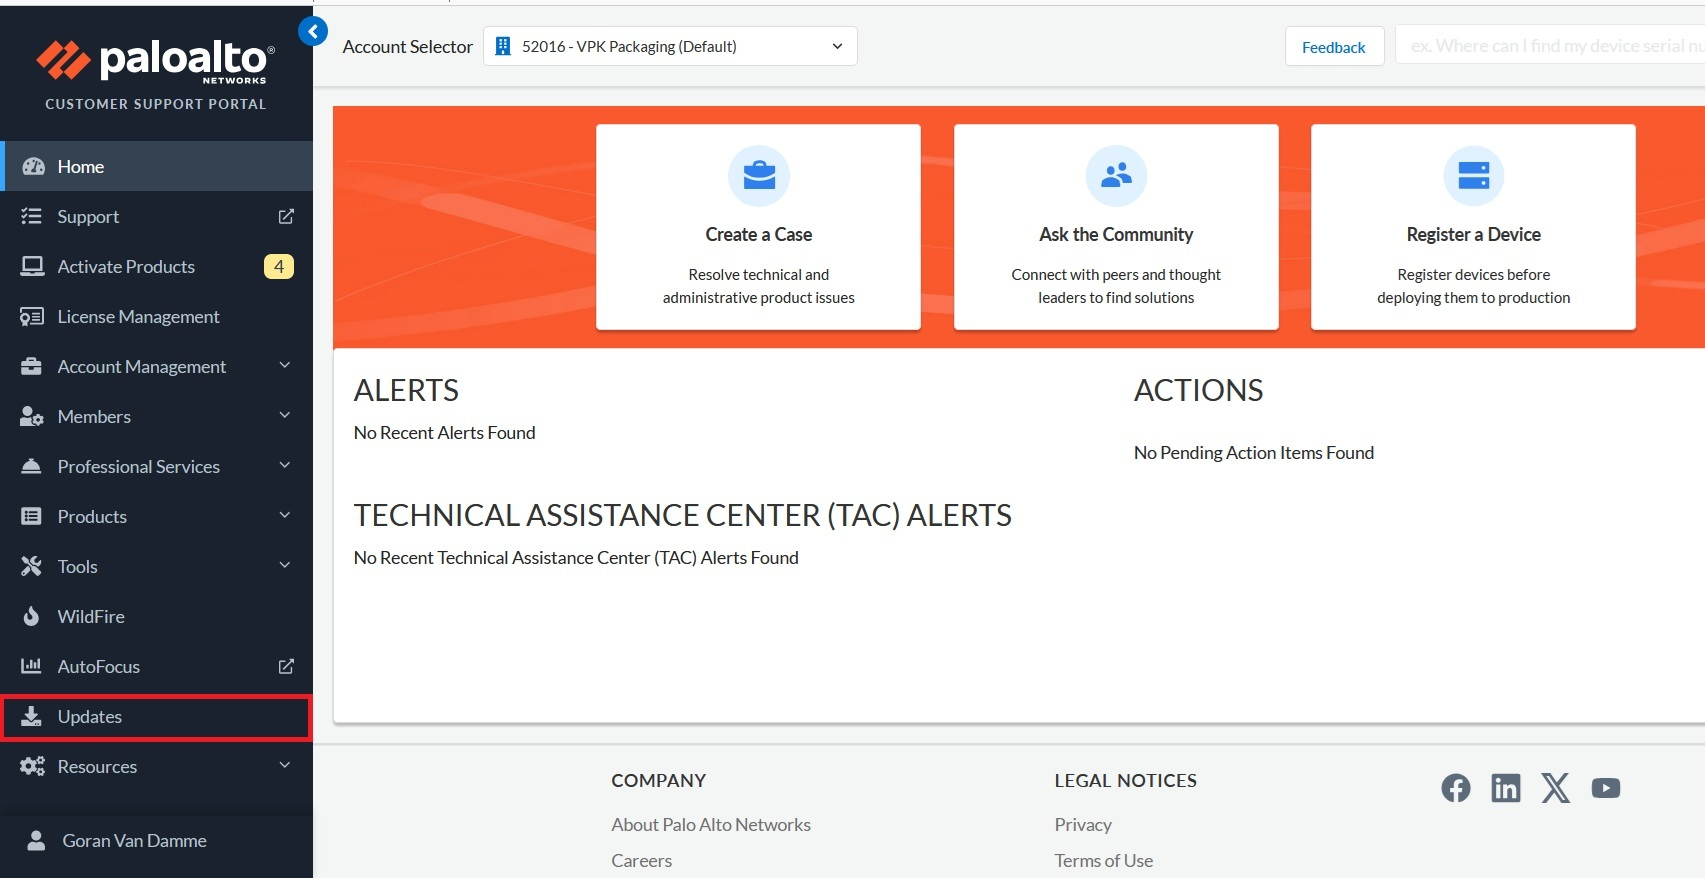
\includegraphics[scale=0.335]{fotos/PA_support_homescreen.jpg}}
    \caption[PA Support Homescreen]{\label{fig:PA_seriesKiezen} Startscherm van de Palo Alto Networks supportwebsite (weergave van mei 2025), met de 'Updates' optie gemarkeerd.}
\end{figure}



\subsection{Downloaden van de correcte PAN-OS versies.}
\label{punt:DownloadenCorrectePanVersie}

Het downloaden van de juiste softwareversie vereist enkele voorbereidende stappen. Allereerst moet worden vastgesteld tot welke serie de gebruikte Palo Alto firewall behoort. In deze POC betreft het een Palo Alto PA-440 firewall, onderdeel van de PA-400 series. Daarnaast moet het upgrade pad bekend zijn, zoals eerder beschreven in punt \ref{punt:BepalenVanHetUpgradePad}.

Selecteer in het contenttype keuzemenu de optie die past bij de series van firewall die geupgrade moet worden, zoals te zien is in figuur \ref{fig:PA_seriesKiezen}. Vervolgens wordt een overzicht weergegeven van alle beschikbare preferred releases van PAN-OS. Bij het kiezen van een preferred release wordt aanbevolen altijd de meest recente versie te selecteren. In het kader van deze POC is het uiteindelijke doel een upgrade naar versie 11.1.6-h3. Deze versie moet dan ook worden gedownload.

Het is belangrijk om te noteren dat alle tussenliggende versies binnen het upgrade pad eveneens moeten worden gedownload. Hiervoor kan in het keuzemenu bij ‘Release type selector’ de optie ‘Other’ worden geselecteerd. Dit geeft een overzicht van alle beschikbare versies, zodat de versies binnen het specifieke upgrade pad handmatig kunnen worden gedownload.


\begin{figure}[H]
    \centering
    \fbox{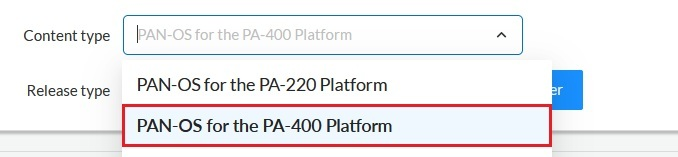
\includegraphics[scale=0.5]{fotos/PA_seriesKiezen.jpg}}
    \caption[PA Support Homescreen]{\label{fig:PA_seriesKiezen} Weergave van de 'Release type' optie.}
\end{figure}


\section{Uitvoeren van de PAN-OS upgrade}
\subsection{Identificeren van Active en Passive firewall.}
\label{punt:DownloadenCorrectePanVersie}

Voordat het mogelijk is om de firmware van een HA firewall pair te upgraden, moet worden gecontroleerd welke firewall momenteel actief is en welke passief. Indien het paneel 'High Availability' niet zichtbaar is op het Dashboard van de firewall, kan dit worden toegevoegd door naar het Dashboard te navigeren en te klikken op:  
“Widgets” \rightarrow “System”  \rightarrow “High Availability”. Voer dit uit op beide firewalls.
Door dit uit te voeren zou je de High Availability widget op het startscherm van de Palo Alto moeten terugvinden zoals getoond in figuur \ref{fig:PA_High_Availability_Widget}.

\begin{figure}[H]
    \centering
    \fbox{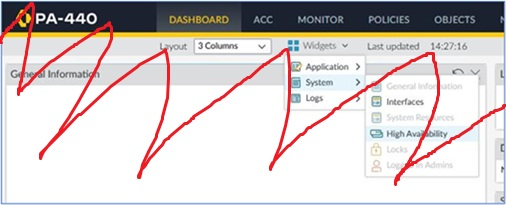
\includegraphics[scale=0.7]{fotos/HA_Widget.jpg}}
    \caption[PA High Availability Widget]{\label{fig:PA_High_Availability_Widget} Weergave van gekozen opties om de HA widget op het dashboard te tonen.}
\end{figure}

Omdat nu de verschillende HA widget zichtbaar is op het scherm hebben we een overzicht over de verschillende HA waardes die ingesteld zijn op de firewall. Zoals te zien is op figuur \ref{fig:PA_High_Availability_Dashboard}. In 

\begin{figure}[H]
    \centering
    \fbox{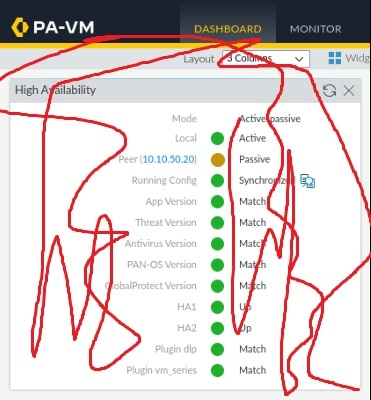
\includegraphics[scale=0.7]{fotos/PA_HADashboard.jpg}}
    \caption[PA High Availability Dashboard]{\label{fig:PA_High_Availability_Dashboard} Weergave van het HA dashboard op het startscherm van de Palo Alto firewall.}
\end{figure}

\subsubsection{Verschillende termen op het HA dashboard}


\begin{table}[h!]
    \centering
    \resizebox{\textwidth}{!}{%
        \begin{tabular}{|l|l|l|}
            \hline
            \textbf{Term} & \textbf{Status} & \textbf{Opties} \\
            \hline
            Mode & Toont HA opstelling & Active-Passive / Active-Active \\
            \hline
            Active-passive & Toont de huidige rol van het apparaat & Active / Passive \\
            \hline
            Peer & IP adres van de HA peer & x.x.x.x \\
            \hline
            Running Config & Configuratiesynchronisatie & Synchronized / Not synchronized \\
            \hline
            App Version & Versie App-ID handtekeningen & Match / Mismatch \\
            \hline
            Threat Version & Versie dreigingssignaturen & Match / Mismatch \\
            \hline
            Antivirus Version & Versie antivirus-handtekeningen & Match / Mismatch \\
            \hline
            PAN-OS Version & Versie van het besturingssysteem & Match / Mismatch \\
            \hline
            GlobalProtect Version & Versie van GlobalProtect & Match / Mismatch \\
            \hline
            HA1 & Status van HA1-kanaal & Up / Down \\
            \hline
            HA2 & Status van HA2-kanaal & Up / Down \\
            \hline
            Plugin dlp & Status van DLP plugin & Match / Mismatch \\
            \hline
            Plugin vm\_series & Status van VM-series plugin & Niet van toepassing op fysieke firewalls \\
            \hline
        \end{tabular}%
    }
    \caption{Overzicht van belangrijke statusinformatie in de High Availability widget.}
    \label{tab:HA_widget_overzicht}
\end{table}

\subsubsection{Verschillende stappen in het upgradeproces van een HA firewall pair}

Het upgraden van een Palo Alto HA firewall pair vereist een zorgvuldige planning en uitvoering om downtime te voorkomen. Er zijn specifieke stappen die in een vaste volgorde moeten worden gevolgd. Afwijken van deze volgorde kan leiden tot onverwachte onderbrekingen in de dienstverlening. Onderstaande stappen beschrijven de aanbevolen procedure in grote lijnen:

\begin{enumerate}
    \item Voer de upgrade uit op de firewall die zich momenteel in de \textit{passive mode} bevindt.
    \item Voer een \textit{failover} uit zodat de geüpgradede firewall de \textit{active} rol overneemt.
    \item Voer de upgrade uit op de firewall die nog niet is bijgewerkt en momenteel in \textit{passive mode} staat.
\end{enumerate}

\subsection{Bepalen van de actieve firewall}
Het identificeren van de actieve en passieve firewall binnen een HA pair is eenvoudig. Open het dashboard van beide firewalls en controleer de \textit{HA widget}. De firewall waarbij naast de lokale waarde ‘Passive’ wordt weergegeven zoals getoond in figuur \ref{fig:PassiveFirewallHADashboard}, is op dat moment de passieve firewall. Deze firewall wordt als eerste geüpgraded. 

\begin{figure}[H]
    \centering
    \fbox{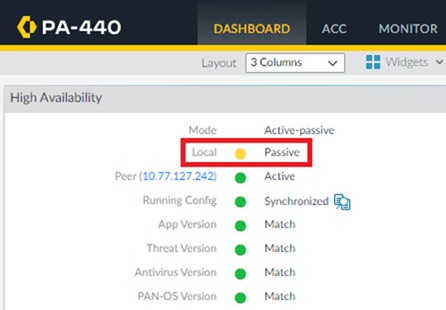
\includegraphics[scale=0.7]{fotos/PassiveFirewallHADashboard.jpg}}
    \caption[PA High Availability Dashboard Passive Firewall]{\label{fig:PassiveFirewallHADashboard} Weergave van het HA dashboard van de Passive firewall.}
\end{figure}


